\chapter{Katalisis Organologam: Tahap Elementer dan Siklus}\label{ch:b2:catalytic-cycles}

Beberapa miligram garam paladium dapat menyambungkan dua cincin \omterm{def:b2:huckel:aromatic}{aromatik}
dalam labu yang berisi berkilo-kilogram pereaksi: atom logam yang sama
mengerjakan tugas itu ribuan kali, dan kembali ke keadaan awalnya setelah
setiap putaran. Bagaimana hal itu terjadi diceritakan oleh sebuah \omterm{def:b2:catalytic-cycles:cycle}{siklus
katalitik}, yaitu urutan tertutup dari segelintir tahap elementer. Jenis
tahap itu hanya sedikit, dan masing-masing mengubah bilangan oksidasi,
jumlah elektron, dan jumlah ligan logam dengan cara yang tetap. Dengan
perhitungan elektron pada \cref{ch:b2:coordination-complexes}, sebuah
siklus dapat dibaca, diperiksa, dan kadang-kadang diramalkan.

\begin{recall}
\Cref{ch:b2:coordination-complexes}: bilangan oksidasi, $d^n$, \omterm{def:b2:coordination-complexes:electron-count}{jumlah elektron valensi},
\omterm{def:b2:coordination-complexes:electron-count}{aturan 18 elektron}, \omterm{def:b2:coordination-complexes:hapticity}{hapisitas}. \Cref{ch:b2:ligand-field}: ligan akseptor $\pi$ dan
\omterm{def:b2:ligand-field:pi-ligands}{donasi balik}. Jilid Tahun 1: katalis, katalisis homogen, tahap elementer,
tahap penentu laju, senyawa organologam, bilangan oksidasi.
\end{recall}

\begin{omfigure}
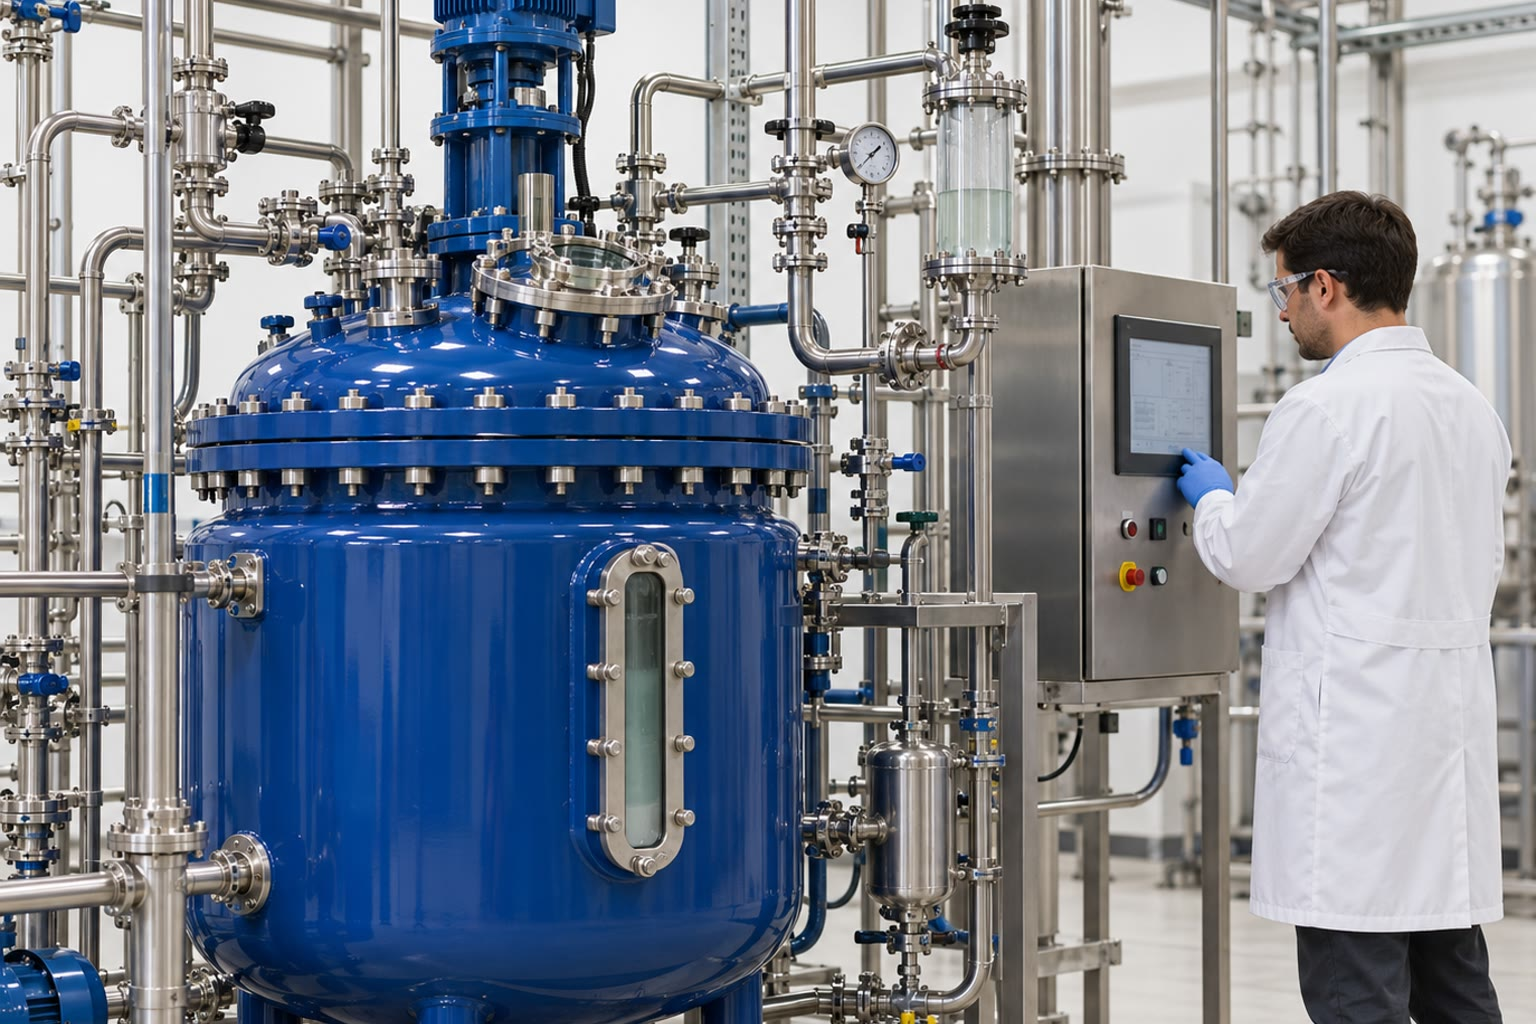
\includegraphics[width=0.62\linewidth]{images/book3/ai/b2-20-pilot-plant.jpg}

{\small Sebuah pabrik percontohan kimia proses: reaktor baja berlapis kaca,
tempat sebuah reaksi kopling terkatalisis ditingkatkan skalanya dari labu
sebelum produksi.}
\end{omfigure}

\section{Bahasa kompleks organologam}

Elektron kompleks organologam dihitung seperti pada \cref{met:b2:coordination-complexes:electron-count},
dengan beberapa ligan tambahan: hidrida \ce{H-} dan anion alkil atau aril
\ce{R-} masing-masing memberikan dua elektron dan dihitung $-1$ dalam
bilangan oksidasi; \ce{CO}, fosfina \ce{PR3}, dan
$\eta^2$-alkena memberikan dua elektron dan dihitung 0; halida \ce{X-}
memberikan dua dan dihitung
$-1$.

\begin{definition}[Kompleks tak jenuh]\label{def:b2:catalytic-cycles:unsaturated}
Sebuah \emph{kompleks tak jenuh koordinatif}\index{kompleks tak jenuh koordinatif}
mempunyai kurang dari 18 elektron valensi (sering 16) dan dapat mengikat
ligan lain: kompleks itu mempunyai sebuah \emph{situs kosong}\index{situs kosong},
yaitu posisi dalam \omterm{def:b2:coordination-complexes:coordination-sphere}{bola koordinasinya} yang bebas untuk menerima donor dua
elektron.
\end{definition}

Kompleks $d^8$ bujur sangkar planar dari rodium(I), iridium(I), paladium(II),
dan platina(II) adalah kompleks 16 elektron; bisfosfina paladium(0) \ce{PdL2}
mempunyai 14. Kompleks-kompleks semacam itu adalah spesies aktif sebagian
besar \omterm{def:b2:catalytic-cycles:cycle}{siklus katalitik}.

\begin{method}[Menghitung kompleks organologam]\label{met:b2:catalytic-cycles:count-organometallic}
\begin{enumerate}
  \item Daftarlah ligan-ligannya: anionik (\ce{H-}, \ce{R-}, \ce{X-}, \ce{C5H5-}) dan netral
        (\ce{CO}, \ce{PR3}, alkena, pelarut).
  \item Bilangan oksidasi = muatan kompleks $-$ jumlah muatan ligan anionik.
  \item $n = g -$ bilangan oksidasi; jumlah elektron = $n + 2 \times$(banyaknya donor dua elektron)
        $+$ 6 per $\eta^5$-\ce{C5H5-}.
  \item Bilangan koordinasi = banyaknya posisi ligan yang terisi.
\end{enumerate}
\end{method}

\section{Pertukaran ligan, adisi oksidatif, eliminasi reduktif}

\begin{definition}[Pertukaran ligan]\label{def:b2:catalytic-cycles:ligand-exchange}
Yang disebut \emph{pertukaran ligan}\index{pertukaran ligan} adalah tahap
elementer yang menggantikan sebuah ligan dalam \omterm{def:b2:coordination-complexes:coordination-sphere}{bola koordinasi} dengan ligan
lain; tahap ini tidak mengubah bilangan oksidasi dan, secara keseluruhan,
tidak mengubah jumlah elektron. Mekanismenya dipelajari dalam jilid Tahun 3.
\end{definition}

\begin{definition}[Adisi oksidatif dan eliminasi reduktif]\label{def:b2:catalytic-cycles:oxidative-addition}
Dalam \emph{adisi oksidatif}\index{adisi oksidatif}, sebuah molekul A--B
beradisi pada pusat logam dengan memutus ikatan A--B-nya dan membentuk
ikatan M--A dan M--B. Yang disebut
\emph{eliminasi reduktif}\index{eliminasi reduktif} adalah tahap
kebalikannya: dua ligan A dan B, yang saling cis, bergabung menjadi A--B dan
meninggalkan logam.
\end{definition}

\begin{proposition}[Menghitung adisi oksidatif]\label{prop:b2:catalytic-cycles:oa}
\omterm{def:b2:catalytic-cycles:oxidative-addition}{Adisi oksidatif} menaikkan bilangan oksidasi logam sebesar 2, \omterm{def:b2:coordination-complexes:electron-count}{jumlah elektron
valensinya} sebesar 2, dan bilangan koordinasinya sebesar 2; \omterm{def:b2:catalytic-cycles:oxidative-addition}{eliminasi
reduktif} menurunkan masing-masing sebesar 2.
\end{proposition}

\begin{proof}
A dan B dihitung sebagai anion (\ce{H-}, \ce{R-}, \ce{X-}) setelah terikat:
dua ligan anionik baru menaikkan bilangan oksidasi sebesar 2 dan menurunkan
$n$ sebesar 2; keduanya memberikan dua pasang, $+4$
elektron; jumlah elektron berubah sebesar $-2 + 4 = +2$. Dua posisi kini
terisi. Tahap kebalikannya membalik setiap perubahan.
\end{proof}

\begin{example}[Kompleks Vaska]\label{ex:b2:catalytic-cycles:vaska}
\ce{[IrCl(CO)(PPh3)2]}, bujur sangkar planar: iridium(I), $d^8$, 16 elektron,
berkoordinasi empat. Kompleks ini mengadisi dihidrogen:
\ce{[IrH2Cl(CO)(PPh3)2]}, iridium(III), $d^6$, 18 elektron, oktahedral,
dengan kedua hidrida cis.
\end{example}

\section{Insersi, eliminasi, transmetalasi}

\begin{definition}[Insersi dan eliminasi $\beta$-hidrida]\label{def:b2:catalytic-cycles:insertion}
Dalam \emph{insersi migrasi}\index{insersi migrasi}, sebuah ligan tak jenuh
(alkena, \ce{CO}) yang terikat pada logam menyisip ke dalam ikatan M--H atau
M--C yang cis: \ce{M-H} dan alkena menghasilkan alkil \ce{M-CH2-CH2-H};
\ce{M-R} dan \ce{CO} menghasilkan asil \ce{M-C(=O)R}.
Yang disebut \emph{eliminasi $\beta$-hidrida}\index{eliminasi beta-hidrida@eliminasi $\beta$-hidrida}
adalah kebalikan insersi alkena: sebuah hidrogen pada karbon $\beta$ terhadap
logam berpindah ke logam, sambil melepaskan alkena.
\end{definition}

\begin{proposition}[Menghitung insersi]\label{prop:b2:catalytic-cycles:insertion}
\omterm{def:b2:catalytic-cycles:insertion}{Insersi migrasi} mempertahankan bilangan oksidasi dan menurunkan jumlah
elektron sebesar 2 (satu posisi ligan dibebaskan); eliminasi $\beta$-hidrida
menaikkan jumlah itu sebesar 2.
\end{proposition}

\begin{proof}
Sebelum: \ce{H-} (atau \ce{R-}, anionik) dan alkena (netral), dua ligan,
empat elektron. Sesudah: satu alkil (anionik), dua elektron. Muatan
anioniknya tidak berubah: bilangan oksidasinya sama; dua elektron dan satu
posisi hilang.
\end{proof}

\begin{proposition}[Syarat eliminasi $\beta$-hidrida]\label{prop:b2:catalytic-cycles:beta-h}
Sebuah alkil logam mengalami eliminasi $\beta$-hidrida hanya jika alkil itu
membawa hidrogen pada karbon $\beta$-nya dan logamnya mempunyai \omterm{def:b2:catalytic-cycles:unsaturated}{situs kosong}
yang cis terhadap alkil itu.
\end{proposition}

\begin{proof}[Argumen]
Tahap ini melalui susunan beranggota empat M--C$_\alpha$--C$_\beta$--H tempat
hidrogen mencapai logam: tahap ini memerlukan hidrogen itu, dan posisi
kosong di sebelah alkil untuk menerimanya. Gugus metil, benzil, neopentil,
dan aril, yang tidak mempunyai hidrogen $\beta$
yang dapat mencapai logam, stabil terhadap tahap ini.
\end{proof}

\begin{definition}[Transmetalasi]\label{def:b2:catalytic-cycles:transmetalation}
Yang disebut \emph{transmetalasi}\index{transmetalasi} memindahkan sebuah
gugus organik dari satu logam (atau metaloid: boron, seng, timah) ke logam
lain, biasanya sebagai pertukaran dengan halida.
\end{definition}

\begin{omfigure}
\begin{tikzpicture}[font=\small, >={Stealth}]
  \tikzset{omstepar/.style={->, thick}}
  \foreach \y/\l/\r/\top/\bot/\rev in {
      0/{$\mathrm{L}_n\mathrm{M}$}/{$\mathrm{L}_n\mathrm{M(A)(B)}$}/{+ A--B}/{adisi oksidatif}/{eliminasi reduktif},
      -1.5/{$\mathrm{L}_n\mathrm{M(H)(CH_2{=}CH_2)}$}/{$\mathrm{L}_n\mathrm{M{-}CH_2CH_3}$}/{}/{insersi migrasi}/{eliminasi $\beta$-hidrida},
      -3.0/{$\mathrm{L}_n\mathrm{M(X)(R)}$}/{$\mathrm{L}_n\mathrm{M(R)(R')}$}/{+ R$'$--[B], $-$ X--[B]}/{transmetalasi}/{},
      -4.5/{$\mathrm{L}_n\mathrm{M(X)}$}/{$\mathrm{L}_n\mathrm{M(X)(L')}$}/{+ L$'$}/{pertukaran atau pengikatan ligan}/{}} {
    \node[cyclenode, anchor=east] (l) at (0,\y) {\l};
    \node[cyclenode, anchor=west] (r) at (5.2,\y) {\r};
    \draw[omstepar] ($(l.east)+(0.1,0.08)$) -- ($(r.west)+(-0.1,0.08)$) node[midway, above, font=\scriptsize] {\top};
    \node[font=\scriptsize, anchor=north] at (2.6,\y-0.02) {\bot};
    \node[font=\scriptsize, black!55, anchor=west] at (5.2,\y-0.5) {\rev};
  }
\end{tikzpicture}

{\small Tahap-tahap elementer katalisis organologam. \omterm{def:b2:catalytic-cycles:oxidative-addition}{Adisi oksidatif}:
bilangan oksidasi, jumlah elektron, dan bilangan koordinasi $+2$; \omterm{def:b2:catalytic-cycles:oxidative-addition}{eliminasi
reduktif}: $-2$. \omterm{def:b2:catalytic-cycles:insertion}{Insersi migrasi}: jumlah elektron $-2$, bilangan oksidasi
tetap; eliminasi $\beta$-hidrida: kebalikannya. \omterm{def:b2:catalytic-cycles:transmetalation}{Transmetalasi}: sebuah gugus
organik berpindah ke logam dari boron, seng, atau timah.}
\end{omfigure}

\section{Membaca siklus katalitik}

\begin{definition}[Siklus katalitik]\label{def:b2:catalytic-cycles:cycle}
Yang disebut \emph{siklus katalitik}\index{siklus katalitik} adalah urutan
tertutup tahap-tahap elementer yang mengonsumsi pereaksi, melepaskan produk,
dan meregenerasi kompleks pertamanya. Senyawa yang ditambahkan ke dalam
reaksi, yang berubah menjadi kompleks pertama siklus itu, disebut
\emph{prakatalis}\index{prakatalis}. Yang disebut \emph{bilangan
perputaran}\index{bilangan perputaran} (TON) adalah jumlah produk yang
terbentuk per jumlah katalis; \emph{frekuensi
perputaran}\index{frekuensi perputaran} (TOF) adalah bilangan perputaran per
satuan waktu.
\end{definition}

\begin{proposition}[Persamaan keseluruhan]\label{prop:b2:catalytic-cycles:cycle-sum}
Jumlah tahap-tahap sebuah \omterm{def:b2:catalytic-cycles:cycle}{siklus katalitik} adalah persamaan reaksi yang
dikatalisis: setiap kompleks logam muncul sekali sebagai produk dan sekali
sebagai pereaksi, dan saling meniadakan.
\end{proposition}

\begin{proof}
Karena siklusnya tertutup, setiap zat antara dibentuk oleh satu tahap dan
dikonsumsi oleh tahap berikutnya; jika tahap-tahap itu dijumlahkan,
spesies-spesies ini muncul di kedua ruas dan saling meniadakan. Yang tersisa
adalah spesies yang masuk dari luar (pereaksi) dan yang keluar (produk).
\end{proof}

\begin{method}[Membaca siklus]\label{met:b2:catalytic-cycles:read-cycle}
\begin{enumerate}
  \item Untuk setiap kompleks, hitunglah bilangan oksidasi, jumlah elektron,
        dan bilangan koordinasinya.
  \item Namailah setiap tahap dari perubahannya ($+2/+2/+2$: \omterm{def:b2:catalytic-cycles:oxidative-addition}{adisi oksidatif}; jumlah
        elektron $-2$ pada bilangan oksidasi tetap: insersi; dan seterusnya).
  \item Periksalah bahwa tidak ada kompleks yang melampaui 18 elektron dan
        bahwa tahap yang memerlukan \omterm{def:b2:catalytic-cycles:unsaturated}{situs kosong} berawal dari kompleks tak jenuh.
  \item Jumlahkan tahap-tahapnya: jumlahnya harus berupa persamaan keseluruhan.
\end{enumerate}
\end{method}

\begin{omfigure}
\begin{tikzpicture}[font=\small, >={Stealth}]
  \node[cyclenode] (n1) at (90:2.3) {\ce{[RhCl(PPh3)2]}\\ Rh(I), 14 e};
  \node[cyclenode] (n2) at (0:3.4) {\ce{[RhH2Cl(PPh3)2]}\\ Rh(III), 16 e};
  \node[cyclenode] (n3) at (270:2.3) {\ce{[RhH2Cl(PPh3)2(RCH=CH2)]}\\ Rh(III), 18 e};
  \node[cyclenode] (n4) at (180:3.4) {\ce{[RhH(CH2CH2R)Cl(PPh3)2]}\\ Rh(III), 16 e};
  \draw[cyclearc] (n1) to[bend left=20] node[cyclelabel, below left] {adisi\\ oksidatif} (n2);
  \draw[cyclearc] (n2) to[bend left=20] node[cyclelabel, left=12pt] {pengikatan\\ alkena} (n3);
  \draw[cyclearc] (n3) to[bend left=20] node[cyclelabel, above right] {insersi\\ migrasi} (n4);
  \draw[cyclearc] (n4) to[bend left=20] node[cyclelabel, below right] {eliminasi\\ reduktif} (n1);
  \draw[cyclein] (4.6,2.3) node[right] {\ce{H2}} -- (2.6,1.75);
  \draw[cyclein] (4.6,-2.3) node[right] {alkena} -- (2.6,-1.75);
  \draw[cycleout] (-2.6,1.75) -- (-4.6,2.3) node[left] {alkana};
  \node[font=\scriptsize, align=center, black!60] at (0,-0.05) {prakatalis\\ \ce{[RhCl(PPh3)3]}\\ melepas \ce{PPh3}};
\end{tikzpicture}

{\small Hidrogenasi alkena dengan katalis Wilkinson, disederhanakan
(pertukaran fosfina dan pelarut tidak ditampilkan). Jumlah keempat tahap itu
adalah $\ce{RCH=CH2 + H2 -> RCH2CH3}$; kompleks-kompleks rodium saling
meniadakan.}
\end{omfigure}

\begin{omfigure}
\begin{tikzpicture}[font=\small, >={Stealth}]
  \node[cyclenode] (s1) at (90:2.3) {\ce{PdL2}\\ Pd(0), 14 e};
  \node[cyclenode] (s2) at (0:3.4) {\ce{[ArPd(Br)L2]}\\ Pd(II), 16 e};
  \node[cyclenode] (s3) at (270:2.3) {$[\mathrm{ArPd(Ar')L_2}]$\\ Pd(II), 16 e};
  \draw[cyclearc] (s1) to[bend left=25] node[cyclelabel, below left] {adisi\\ oksidatif} (s2);
  \draw[cyclearc] (s2) to[bend left=25] node[cyclelabel, above left] {transmetalasi} (s3);
  \draw[cyclearc] (s3) to[bend left=35] node[cyclelabel, right] {eliminasi\\ reduktif} (s1);
  \draw[cyclein] (4.8,2.2) node[right] {\ce{Ar-Br}} -- (2.6,1.6);
  \draw[cyclein] (5.4,-0.9) node[right, align=left] {$\mathrm{Ar'B(OH)_2}$\\ + basa} -- (3.3,-1.2);
  \draw[cycleout] (2.3,-2.0) -- (4.4,-2.9) node[right] {\ce{Br-}, \ce{B(OH)3}};
  \draw[cycleout] (-1.75,-0.4) -- (-4.2,-0.4) node[left] {$\mathrm{Ar{-}Ar'}$};
\end{tikzpicture}

{\small Kopling Suzuki, disederhanakan. Paladium(0) mengadisi aril bromida;
basa mengubah asam boronat menjadi borat, yang memindahkan gugus arilnya ke
paladium; kedua aril, yang cis, dieliminasi sebagai biaril, sambil
meregenerasi paladium(0).}
\end{omfigure}

Dalam reaksi Heck, kompleks aril--paladium yang terbentuk melalui \omterm{def:b2:catalytic-cycles:oxidative-addition}{adisi
oksidatif} mengikat alkena alih-alih borat; \omterm{def:b2:catalytic-cycles:insertion}{insersi migrasi} menempatkan aril
pada alkena, dan eliminasi $\beta$-hidrida melepaskan alkena tersubstitusi
(biasanya isomer trans) dan sebuah hidrida paladium, yang darinya basa
mengambil \ce{HBr} untuk meregenerasi paladium(0).

Hidroformilasi, yaitu adisi \ce{H2} dan \ce{CO} pada alkena yang menghasilkan
aldehida, berlangsung dengan hidrida kobalt atau rodium melalui insersi
alkena, insersi \ce{CO} ke dalam ikatan logam--alkil, \omterm{def:b2:catalytic-cycles:oxidative-addition}{adisi oksidatif} \ce{H2},
dan \omterm{def:b2:catalytic-cycles:oxidative-addition}{eliminasi reduktif} aldehida. Arah insersi pertama menentukan produknya:
logam pada karbon ujung menghasilkan aldehida linear, pada karbon dalam
menghasilkan aldehida bercabang; fosfina yang meruah lebih menyukai produk
linear.

\begin{history}[Kopling silang]
\begin{minipage}[t]{0.36\linewidth}
\vspace{0pt}
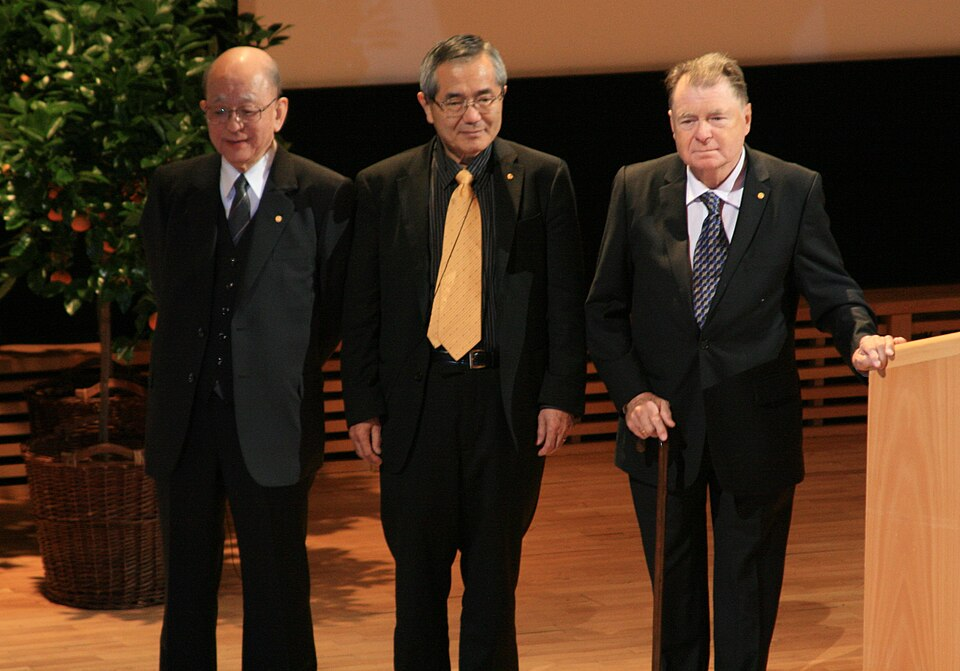
\includegraphics[width=\linewidth]{images/book3/nobel-2010.jpg}
\end{minipage}\hfill
\begin{minipage}[t]{0.6\linewidth}
\vspace{0pt}
Kopling-kopling terkatalisis paladium dari aril dan vinil halida dengan
alkena (Richard Heck, sejak 1968), dengan pereaksi organoseng (Ei-ichi
Negishi, 1977), dan dengan senyawa organoboron (Akira Suzuki, 1979) membuat
penyambungan dua kerangka karbon menjadi pekerjaan rutin; reaksi-reaksi itu
kini termasuk yang paling banyak dipakai dalam pembuatan obat dan material.
Hadiah Nobel Kimia dianugerahkan kepada ketiganya pada tahun 2010. (Foto:
Suzuki, Negishi, dan Heck, dari kiri ke kanan, 2010; BloodIce, CC BY-SA 4.0,
Wikimedia Commons.)
\end{minipage}
\end{history}

\begin{proposition}[Perputaran]\label{prop:b2:catalytic-cycles:tof}
Dengan $n_P$ jumlah produk yang terbentuk dalam waktu $t$ oleh sejumlah $n_{\text{kat}}$ katalis,
$\mathrm{TON} = n_P/n_{\text{kat}}$ dan \omterm{def:b2:catalytic-cycles:cycle}{frekuensi perputaran} rata-ratanya adalah $\mathrm{TOF} =
\mathrm{TON}/t$.
\end{proposition}

\begin{proof}
Setiap putaran siklus menghasilkan satu molekul produk per atom logam;
banyaknya putaran yang dilakukan setiap atom rata-rata adalah $n_P/n_{\text{kat}}$,
dan laju perputarannya adalah bilangan itu per satuan waktu.
\end{proof}

\begin{safety}{\ghs[5mm]{GHS05}\,\ghs[5mm]{GHS07}\,\ghs[5mm]{GHS09}}
Paladium(II) etanoat korosif terhadap mata dan beracun bagi kehidupan
akuatik; trifenilfosfina berbahaya dan menyebabkan sensitisasi.
Senyawa-senyawa itu ditimbang di dalam lemari asam, dan residu paladium
dikumpulkan untuk diambil kembali, tidak pernah dibuang ke saluran air.
% ledger: ghs:Pd-acetate, ghs:PPh3, ghs:phenylboronic-acid, ghs:4-bromotoluene
\end{safety}

\section{Latihan}

\begin{exercise}[$\star$]\label{exo:b2:catalytic-cycles:1}
Tuliskan bilangan oksidasi, $d^n$, dan jumlah elektron kompleks Vaska
\ce{[IrCl(CO)(PPh3)2]} sebelum dan sesudah kompleks itu mengadisi \ce{H2}.
\end{exercise}

\begin{exercise}[$\star$]\label{exo:b2:catalytic-cycles:2}
Namailah tahapnya: \ce{[PtCl2(CH3)2(PR3)2] -> [PtCl2(PR3)2] + C2H6}; \ce{[Pd(Ph)Br(PR3)2] +
CH2=CH2 -> [Pd(CH2CH2Ph)Br(PR3)] + PR3}.
\end{exercise}

\begin{exercise}[$\star$]\label{exo:b2:catalytic-cycles:3}
Sebuah reaksi memakai \qty{0.020}{mmol} katalis dan menghasilkan
\qty{15.0}{mmol} produk dalam \qty{3.0}{h}. Hitunglah TON dan TOF rata-ratanya.
\end{exercise}

\begin{exercise}[$\star$]\label{exo:b2:catalytic-cycles:4}
Jumlahkan ketiga tahap siklus Suzuki dan periksalah bahwa paladium saling meniadakan.
\end{exercise}

\begin{exercise}[$\star\star$]\label{exo:b2:catalytic-cycles:5}
Kompleks alkil paladium manakah di antara berikut ini yang dapat mengalami
eliminasi $\beta$-hidrida: \ce{Pd-CH3}, \ce{Pd-CH2CH3}, \ce{Pd-CH2C(CH3)3},
\ce{Pd-CH2Ph}, \ce{Pd-CH(CH3)2}?
\end{exercise}

\begin{exercise}[$\star\star$]\label{exo:b2:catalytic-cycles:6}
Ramalkan produk reaksi Heck iodobenzena dengan metil propenoat, beserta
geometrinya.
\end{exercise}

\begin{exercise}[$\star\star$]\label{exo:b2:catalytic-cycles:7}
Tuliskan aldehida linear dan bercabang yang terbentuk melalui hidroformilasi
propena, dan jelaskan insersi mana yang menghasilkan masing-masing.
\end{exercise}

\begin{exercise}[$\star\star$]\label{exo:b2:catalytic-cycles:8}
Mengapa \ce{[RhCl(PPh3)3]} hanya dapat mengadisi \ce{H2} setelah melepaskan
sebuah fosfina, sedangkan \ce{[RhCl(PPh3)2]} langsung mengadisinya?
\end{exercise}

\begin{exercise}[$\star\star$]\label{exo:b2:catalytic-cycles:9}
Dalam kopling Suzuki, mengapa diperlukan basa, dan apa yang dilakukannya pada asam boronat?
\end{exercise}

\begin{exercise}[$\star\star\star$]\label{exo:b2:catalytic-cycles:10}
Sebuah siklus yang diusulkan untuk hidrogenasi alkena pada kompleks $d^8$
\ce{ML3X} (16 e) berawal dengan pengikatan alkena menjadi kompleks 20
elektron, lalu \omterm{def:b2:catalytic-cycles:oxidative-addition}{adisi oksidatif} \ce{H2}. Temukan kesalahannya dan perbaikilah
urutannya.
\end{exercise}

\begin{exercise}[$\star\star\star$]\label{exo:b2:catalytic-cycles:11}
Jumlah produk sebuah reaksi terkatalisis bertambah menurut $n_P(t) = n_{\max}(1 - \mathrm e^{-t/\tau})$
dengan $n_{\max} = \qty{10.0}{mmol}$, $\tau = \qty{40}{min}$, dan \qty{0.010}{mmol}
katalis (data latihan). Hitunglah TOF awal dan TON akhirnya.
\end{exercise}

\begin{exercise}[$\star\star\star$]\label{exo:b2:catalytic-cycles:12}
Usulkan sebuah kopling silang untuk membuat 4-metoksibifenil, dengan memilih
halida dan asam boronatnya, dan tuliskan siklusnya.
\end{exercise}

\section{Soal: Membaca Siklus Suzuki}

\begin{problem}[{Soal akhir pekan --- prakatalis dan paladium(0) yang aktif,
adisi oksidatif, transmetalasi, dan eliminasi reduktif dalam kopling Suzuki,
rendemen dan bilangan perputaran, serta reaksi-reaksi samping}]
\label{pb:b2:catalytic-cycles:1}
Percobaan (data latihan): \qty{10.0}{mmol} 4-bromotoluena, \qty{12.0}{mmol}
asam fenilboronat, \qty{20}{mmol} kalium karbonat, \qty{0.050}{mmol}
paladium(II) etanoat, dan \qty{0.10}{mmol} trifenilfosfina dalam campuran
toluena, etanol, dan air, dipanaskan di bawah nitrogen; produk yang
diisolasi: \qty{1.51}{g} 4-metilbifenil. Massa molar (\unit{g/mol}):
4-bromotoluena 171.04, asam fenilboronat 121.93, 4-metilbifenil
168.24, paladium(II) etanoat 224.51.
% ledger: aw:C, aw:H, aw:Br, aw:B, aw:O, aw:Pd

\medskip
\noindent\textbf{Bagian I --- Katalis.}
\begin{enumerate}
  \item Tuliskan bilangan oksidasi dan $d^n$ paladium dalam paladium(II) etanoat.
  \item Di dalam labu, senyawa itu direduksi menjadi \ce{Pd(PPh3)2}. Tuliskan
        bilangan oksidasi, $d^n$, dan jumlah elektronnya.
  \item Mengapa kompleks itu tak jenuh koordinatif?
  \item Mengapa reaksi itu dijalankan di bawah nitrogen?
  \item Apa peran trifenilfosfina yang berlebih?
  \item Apakah paladium(II) etanoat itu katalis atau \omterm{def:b2:catalytic-cycles:cycle}{prakatalis}?
\end{enumerate}

\medskip
\noindent\textbf{Bagian II --- Tahap-tahap.}
\begin{enumerate}[resume]
  \item Tuliskan \omterm{def:b2:catalytic-cycles:oxidative-addition}{adisi oksidatif} 4-bromotoluena dan hitunglah elektron produknya.
  \item Apa yang dilakukan karbonat pada asam fenilboronat?
  \item Tuliskan \omterm{def:b2:catalytic-cycles:transmetalation}{transmetalasinya}.
  \item Mengapa kedua gugus aril harus cis sebelum tahap berikutnya?
  \item Tuliskan \omterm{def:b2:catalytic-cycles:oxidative-addition}{eliminasi reduktifnya} dan hitunglah elektron spesies paladium
        yang terbentuk.
  \item Jumlahkan ketiga tahap itu.
\end{enumerate}

\medskip
\noindent\textbf{Bagian III --- Rendemen dan perputaran.}
\begin{enumerate}[resume]
  \item Pereaksi manakah yang menjadi pembatas?
  \item Hitunglah jumlah produk yang diisolasi.
  \item Hitunglah rendemennya.
  \item Hitunglah kadar katalis dalam mol~\% relatif terhadap bromida.
  \item Hitunglah \omterm{def:b2:catalytic-cycles:cycle}{bilangan perputaran} paladium.
  \item Percobaan itu berlangsung \qty{4.0}{h}. Hitunglah \omterm{def:b2:catalytic-cycles:cycle}{frekuensi perputaran}
        rata-rata per jam.
\end{enumerate}

\medskip
\noindent\textbf{Bagian IV --- Reaksi samping.}
\begin{enumerate}[resume]
  \item Sejumlah bifenil \ce{Ph-Ph} ditemukan. Usulkan bagaimana senyawa itu terbentuk.
  \item Mengapa tidak ada eliminasi $\beta$-hidrida yang mungkin di sini?
  \item Aril klorida bereaksi jauh lebih lambat daripada bromida. Tahap
        manakah yang terhambat?
  \item Apa yang terjadi pada paladium di akhir reaksi, dan mengapa logam itu
        diambil kembali?
  \item Mengapa asam boronat dipakai sedikit berlebih?
  \item Nyatakan \omterm{def:b2:catalytic-cycles:cycle}{bilangan perputaran} paladium dalam percobaan itu.
\end{enumerate}
\end{problem}
